\chapter{基礎圖論}

圖論在演算法這門學科裡佔了十分重要的地位,在競賽中有大約一半的題目會用到圖論的算法與觀念,學著怎麼處理圖,與學習語法一樣重要。\\

\section{名詞解釋}
\subsection{一堆怪東東}

\begin{enumerate}
\item 圖 (Graph):許多頂點與邊的集合,常用 $G(V, E)$ 表示。
\item 頂點 (Vertex):就是頂點 。常用 $v$ 表示。$V$ 就是頂點的集合。
\item 邊 (Edge):連接兩個頂點的東西,可表示成 $e = (u, v)$。$E$ 就是邊的集合。
\item 有向/無向 (Directed/Undirected) 邊:如果 $(u, v)$ 與 $(v, u)$ 代表的是同一條邊,則稱這條邊是無向邊,反之則其中任一條邊為有向邊。
\item 度數 (Degree):一個頂點連接的邊數,即為這個頂點的度數。
\item 入度/出度 (Indegree/Outdegree):若為有向邊,則度數分為入度與出度,分別代表以此頂點為終點與起點的邊數。
\item 鄰接 (Adjacent):如果兩個頂點間有邊連接,則稱這兩個頂點鄰接。
\item 自環:連接相同頂點的邊,即 $(v, v)$。
\item 重邊:兩條或以上連接相同兩個點的邊。
\item 路徑 (Path):一個頂點與邊交錯的序列,滿足每個邊都要連接兩個頂點,且從頂點開始、頂點結束。以 $(v_s, e_1, v_1, e_2, v_2, ..., v_e)$ 表示。
\item 行跡 (Trace):不包含重複邊的路徑。
\item 簡單路徑 (Track):不包含重複頂點的路徑。
\item 迴路 (Circuit):起點與終點為相同頂點的路徑。
\item 環 (Cycle):起點與終點為唯一相同頂點的簡單路徑。
\end{enumerate}

\subsection{各種圖}
\begin{enumerate}
\item 有向圖/無向圖:每條邊都是無向邊的圖稱為無向圖,反之為有向圖。
\item 帶權圖/不帶權圖:有時點上或邊上會有權重,稱為帶權圖。
\item 連通圖:把所有邊變成無向邊後,對於圖上的所有頂點對 $(u, v)$,都存在一個起點為 $u$,終點為 $v$ 的路徑,則稱這個圖為連通圖。
\item 強連通圖:若有向圖上的所有頂點對 $(u, v)$,都存在一個起點為 $u$,終點為 $v$ 的路徑,則稱這個圖為強連通圖。
\item 簡單圖:沒有重邊以及自環的圖,不一定連通。
\item 完全圖:每個頂點都與圖上其他所有頂點鄰接的圖,稱為完全圖。
\item 子圖:今有兩圖 $G(V, E)$ 與 $H$,若對於所有屬於 $H$ 的頂點 $v_i$ 與邊 $e_i$ 皆有 $v_i \in V$ 且 $e_i \in E$ (即 $H$ 內所有頂點與邊都屬於 $G$),則稱 $H$ 是 $G$ 的子圖。
\item 補圖:若圖 $G$ 與圖 $H$ 的頂點集合相同,且兩圖的邊集合聯集為完全圖、交集為空集合,則稱圖 $G$ 與圖 $H$ 互為補圖。
\item 樹:沒有環的連通無向圖稱為樹。
\item 森林:很多樹 (包括一棵) 的聯集稱為森林。
\item 二分圖:如果可以將一張圖的點集分為兩部分,同一部分的任兩點不鄰接,則稱為二分圖。
\item 有向無環圖:簡稱DAG,就是沒有環的有向圖。
\item 稀疏圖/稠密圖:如果邊數十分多(如完全圖),也就是$|E| = O(|V^2|)$,則稱這個圖是稠密圖。若邊數不多($|E| = O(|V|)$ 或 $O(|E|) = O(|V|\log|V|)$),則稱為稀疏圖。
\end{enumerate}

\par 
以上是定義,讓我們看看例圖:

\begin{center}
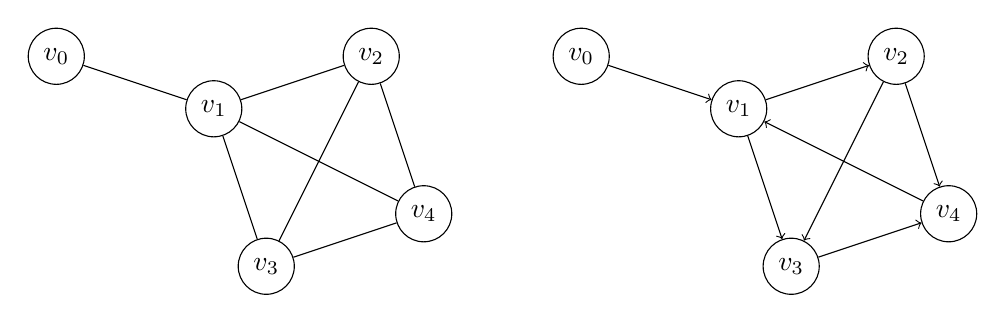
\begin{tikzpicture}[every node/.style={circle,draw=black}]
\node (v1) at (2*0/3,2*5/3) {$v_0$};
\node (v2) at (2*3/3,2*4/3) {$v_1$};
\node (v3) at (2*6/3,2*5/3) {$v_2$};
\node (v4) at (2*4/3,2*1/3) {$v_3$};
\node (v5) at (2*7/3,2*2/3) {$v_4$};
\draw (v1) -- (v2);
\draw (v2) -- (v3);
\draw (v2) -- (v4);
\draw (v3) -- (v5);
\draw (v4) -- (v5);
\draw (v3) -- (v4);
\draw (v2) -- (v5);

\node (v1) at (2*10/3,2*5/3) {$v_0$};
\node (v2) at (2*13/3,2*4/3) {$v_1$};
\node (v3) at (2*16/3,2*5/3) {$v_2$};
\node (v4) at (2*14/3,2*1/3) {$v_3$};
\node (v5) at (2*17/3,2*2/3) {$v_4$};
\draw[->] (v1) -- (v2);
\draw[->] (v2) -- (v3);
\draw[->] (v2) -- (v4);
\draw[->] (v3) -- (v5);
\draw[->] (v4) -- (v5);
\draw[->] (v3) -- (v4);
\draw[<-] (v2) -- (v5);
\end{tikzpicture}
\end{center}
 
我們常用這種方法表示無向圖與有向圖。圖論中的圖上每條邊都是連接兩個頂點,不會交叉。

\section{圖的儲存}
在學習圖論的時候,看到各式各樣的演算法,一定要先確定這個演算法要用什麼方式把圖存下來會比較好處理。這裡提供了三種把圖存在記憶體裡的方式,各自有各自的優缺利弊,在不同圖論算法上有不同應用。\\

通常測資在輸入一張圖時,會先給定兩個數 $n, m$,分別代表頂點數以及邊數,接下來會有 $m$ 行,每行輸入兩個數字 $u_i, v_i$,代表有一條邊從頂點 $u_i$ 連至頂點 $v_i$,如果是帶權圖,那麼每行會輸入三個數,分別代表兩端點以及權重。\\

讓我們把這種輸入格式轉成方便處理的形式吧!

\subsection{鄰接矩陣 (Adjacency Matrix)}
鄰接矩陣是把圖存下來最直覺的想法。考慮一張無向圖:
\begin{center}
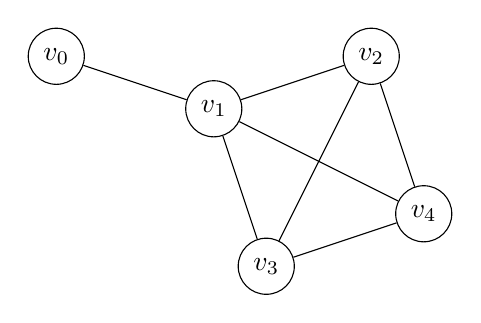
\begin{tikzpicture}[every node/.style={circle,draw=black}]
\node (v1) at (2*0/3,2*5/3) {$v_0$};
\node (v2) at (2*3/3,2*4/3) {$v_1$};
\node (v3) at (2*6/3,2*5/3) {$v_2$};
\node (v4) at (2*4/3,2*1/3) {$v_3$};
\node (v5) at (2*7/3,2*2/3) {$v_4$};
\draw (v1) -- (v2);
\draw (v2) -- (v3);
\draw (v2) -- (v4);
\draw (v3) -- (v5);
\draw (v4) -- (v5);
\draw (v3) -- (v4);
\draw (v2) -- (v5);
\end{tikzpicture}
\end{center}

我們可以將這張圖轉成以下矩陣:
\begin{displaymath}
\begin{bmatrix}
0 & 1 & 0 & 0 & 0\\
1 & 0 & 1 & 1 & 1\\
0 & 1 & 0 & 1 & 1\\
0 & 1 & 1 & 0 & 1\\
0 & 1 & 1 & 1 & 0
\end{bmatrix}
\end{displaymath}

若 $A$ 是一張圖的鄰接矩陣,表示頂點 $i$ 與頂點 $j$ 之間有邊時 $A[i][j] = A[j][i] = 1$,反之 $A[i][j] = 0$。\\

\definition{鄰接矩陣}{
	對於一張圖 $G$,若矩陣 $A$ 滿足:
	\begin{displaymath}
	A[i][j] = 1, \mbox{若邊 $(i, j) \in G$}
	\end{displaymath}
	\begin{displaymath}
	A[i][j] = 0, \mbox{若邊 $(i, j) \notin G$}
	\end{displaymath}
	則稱矩陣 $A$ 是圖 $G$ 的鄰接矩陣。
}

鄰接矩陣也可以處理有向圖以及帶權圖。帶權圖的處理方式十分簡單,就是直接把權重存入鄰接矩陣內;對於一個有向邊 $(i, j)$,則可以用 $A[i][j] = 1, A[i][j] = 0$ 來表示。\\

將輸入轉為鄰接矩陣的方式非常容易,只要將輸入的邊一一填入矩陣即可。
\begin{C++}
int A[MAX_N][MAX_N] = {}; // 初始化為 0
main(){
    int n, m, a, b;
    cin >> n >> m;
    for(int i = 0 ; i < m; i++){
        cin >> a >> b;
        A[a][b] = A[b][a] = 1; // 有邊則改為 1
    }
}
\end{C++}

鄰接矩陣雖然可以在 $O(1)$ 時間檢查兩個頂點之間是否有邊,但是需要用到 $O(|V|^2)$ 的記憶體,所以鄰接矩陣只適合儲存稠密圖。雖然大部分演算法競賽都是以稀疏圖的應用為主,但是鄰接矩陣也有 Floyd Warshall 演算法以及矩陣樹定理等應用。

\section{鄰接串列 (Adjacency List)}
至於稀疏圖,用鄰接串列來儲存是一個比較好的選擇。\\

我們一樣用同一張圖:
\begin{center}
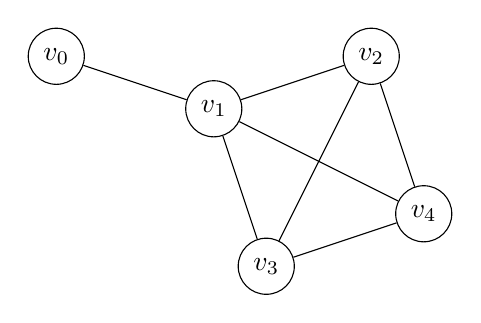
\begin{tikzpicture}[every node/.style={circle,draw=black}]
\node (v1) at (2*0/3,2*5/3) {$v_0$};
\node (v2) at (2*3/3,2*4/3) {$v_1$};
\node (v3) at (2*6/3,2*5/3) {$v_2$};
\node (v4) at (2*4/3,2*1/3) {$v_3$};
\node (v5) at (2*7/3,2*2/3) {$v_4$};
\draw (v1) -- (v2);
\draw (v2) -- (v3);
\draw (v2) -- (v4);
\draw (v3) -- (v5);
\draw (v4) -- (v5);
\draw (v3) -- (v4);
\draw (v2) -- (v5);
\end{tikzpicture}
\end{center}

可以轉換成下列鄰接串列:

\begin{displaymath}
\begin{matrix}
0 & : & 1\\
1 & : & 0 & 2 & 3 & 4\\
2 & : & 1 & 4 & 3\\
3 & : & 1 & 4 & 2\\
4 & : & 2 & 3 & 1\\
\end{matrix}
\end{displaymath}
每個數字 $i$ 後面接的一長串數字就是頂點 $i$ 有連接到的所有頂點的編號。注意串列串的一串數字是無序的,所以檢查兩個點是否有鄰接的最差時間複雜度是 $O(|E|)$。但如果將鄰接串列先排序過,就可以用 $O(\log |E|)$ 的時間二分搜檢查鄰接性了!\\

我們常用一個 \inline{vector<int> L[MAX\_N]} 來實作鄰接串列。 \inline{L[i]} 是一個 \inline{vector},這裡儲存所有與頂點 $i$ 鄰接的所有頂點的編號,如果是帶權圖,就改儲存一個 \inline{pair},表示鄰接頂點的編號與這條邊的權重。以下是將輸入轉成鄰接串列的方法。

\begin{C++}
vector<int> L[MAX_N];
int main(){
    int n, m, a, b;
    cin >> n >> m;
    for(int i = 0 ; i < m; i++){
        cin >> a >> b;
        L[a].push_back(b);
        L[b].push_back(a); // 如果是無向圖必須加上反向邊
    }
}
\end{C++}

鄰接串列應該是演算法競賽裡最常出現的圖儲存方式了,超過半數的問題都是用鄰接串列實現。接下來要提到的 DFS、BFS、最短路徑、二分圖色問題等等,都可以用鄰接串列來完成。

\section{很多邊的東東(?)}
這個東西的英文叫 Edge List,就是一堆邊的集合,這個儲存方式比較簡單也比較接近輸入格式,就是用個 \inline{vector} 將所有邊的兩端點儲存下來,維持原本的輸入格式也可以應用在一些好用的演算法。以下是範例程式碼。

\begin{C++}
vector<pair<int,int>> E;
signed main(){
    int n, m, a, b;
    cin >> n >> m;
    for(int i = 0; i < m; i++){
        cin >> a >> b;
        E.push_back({a, b});
    }
}
\end{C++}

這種儲存方式可以解決最小生成樹的問題,或者實作一些只需要枚舉邊的演算法。

\subsection{其他存圖的方式}
如果讀者有接觸過樹狀資料結構的話,就會知道可以用指標或陣列儲存一棵樹,而樹也是圖的一種,因此如果圖是一棵樹的話,也可以嘗試用樹狀結構的儲存方法。\\

另外,圖還有一種叫做前向星(Forward Star)的儲存方式,不過前向星能做到的事都可以被前面三種所取代,而且實作沒有比較簡單,所以就逐漸被程式競賽淘汰了。

\section{戶口調查時間!}
有了圖之後,我們就到各個頂點看看吧!Let's go!\\

\subsection{深度優先搜尋 (Depth-First-Search, DFS)}
讓我們發揮冒險精神,進入鄰接串列迷宮,往深處探險去吧!\\

終於到了頂點 $s$ 了!這裡還沒被插上探險的標記,讓我們跟居民聊聊天吧。\\

冒險者:叩叩叩,請問一下你們家有多少人?\\

$s$屋主:寒舍只有我與妻子二人,要入屋內坐坐嗎?我這就去殺雞設酒。\\

冒險者:不用了,謝謝。我還要繼續冒險呢!\\

$s$屋主:這是我家私藏的冒險地圖,寫著與這裡鄰接的節點們,祝你好運!\\

冒險者插上了旗子,代表來過這裡的標記,就收起行囊離開前往頂點 $t$ 了。\\

\begin{C++}
vector<int> G[MAX_N];
bool visited[MAX_N] = {};
void dfs(int s){
    // process vertex s
    visited[s] = true;
    for(auto t: G[s]){
        if(!visited[t]) dfs(t);
    }
}
\end{C++}

DFS 是圖論演算法的基礎,通常會使用遞迴來實作,當所有節點都已經被遍歷過時,就達到遞迴的中止條件,可以停止演算法了。在這個程式碼當中 \inline{if(!visited[t])} 的部分在所有節點都已經被遍歷時就不會被呼叫,所以這個遞迴呼叫就一定會被中止。\\

值得注意的是:一次DFS只能拜訪過與起點連通的連通塊的所有節點,如果你想遍歷整張圖的所有節點,必須對所有未被拜訪過的頂點DFS一次,才能確保所有節點都被計算到。這樣雖然最多可能會進行 DFS $O(|V|)$ 次,但是 \inline{visited} 陣列每格最多只會被改成 \inline{true} 一次,所以均攤複雜度仍然是 $O(|V|)$

\begin{C++}
int main(){
    // 在這裡輸入鄰接串列
    for(int i = 0; i < n; i++){
        if(!visited[i]) dfs(i); // 拜訪所有節點
    }
}
\end{C++}

\hint{對於非連通圖的遍歷,一定要寫個 \inline{for} 迴圈對所有節點DFS一次,不然吃WA不瞑目。}

\subsection{廣度優先搜尋 (Breadth-First-Search,BFS)}
相較於深度優先搜尋一路衝到底的精神,廣度優先搜尋比較接近一層一層的探索。\\

出了鄰接串列迷宮之後,冒險者得到了迷宮的全圖。\\

冒險者:這迷宮如此錯綜複雜,我要怎麼知道從起點走到每個頂點要多少時間呢?\\

紫紅神:你可以嘗試遍歷一次地圖,然後帶著一種具有距離標示的旗子。每次幫所有加過標記的點周圍都放上距離多 $1$ 的旗子,這樣就可以卻保距離較近的點先被走到嘍!\\

冒險者:那我要怎麼一次找出所有已標記地點附近的未標記地呢?\\

紫紅神:你應該拿回迷宮的地圖了吧!你可以在標記一個地方的時候,將其附近的頂點全部都放入隊列當中,等到前面還沒標記完的節點被標記後就可以一次找出這個地點的所有附近的未標記地了呢!\\

冒險者:哇!好聰明!我來試試看!\\

\begin{C++}
vector<int> G[MAX_N];
bool visited[MAX_N] = {};
queue<int> que;
void bfs(int s){
    que.push(s);
    while(!que.empty()){
        int v = que.front(), que.pop();
        // process vertex v
        visited[v] = true;
        for(auto t: G[v]){
            if(!visited[t]) que.push(t);
        }
    }
}
\end{C++}

BFS一樣可以對整張圖進行遍歷,不過BFS有一個性質,就是先被處理到的點與起點的距離會比較近,也就是說這種演算法可以計算出起點到圖上任一點的最短路徑長度。讓我們看看以下例題:

\problem{最短路徑}{
	給一張無向連通圖與起終點的編號,求從起點至少需要走過多少邊才能抵達終點。
}

對於這個問題,可以記錄一個陣列 \inline{dist[i]} 代表從起點到頂點 $i$ 的最短路徑,顯然,起點到起點的最短距離是 $0$。然後從起點開始 BFS,每次抵達一個節點 $v$ 時,就將自己附近沒被標記過的節點設成 \inline{dist[v]+1},直到整個圖都被計算過之後,再求取終點的 \inline{dist} 值即可。此外,因為 BFS 可以對整張圖進行遍歷,所以假設起點不動,一次 BFS 就可以算出起點到圖上任意終點的最短路徑。

\begin{C++}
int dist[MAX_N];
int visted[MAX_N];
vector<int> G[MAX_N];
queue<int> que;
void bfs(int s){
    dist[s] = 0;
    que.push(s);
    while(!que.empty()){
        int v = que.front(), que.pop();
        visited[v] = true;
        for(auto t: G[v]){
            if(!visited[t]){
                dist[t] = dist[v] + 1;
                que.push(t);
            }
        }
    }
}
\end{C++}

\section{完全搜尋可以幹嘛}
以下用一些例題來舉例說明完全搜尋的用處吧!\\

\problem{新手訓練系列 \~{} 圖論 (ZJ a290)}{
	給一張有向圖與頂點 $A, B$,求是否可以從 $A$ 通過圖上的邊抵達頂點 $B$。$(|V|\leq 800, |E|\leq 10000)$
}

這題是個暖身題,十分容易。就是從頂點 $A$ 開始 DFS,最後檢查 \inline{visited[B]} 是否為真就行了,輕輕鬆鬆。\\

\problem{最佳路徑 (99北基區資訊能競p4, ZJ d908)}{
	給一張有向且帶邊權的圖,以及起點邊號,求從起點開始的所有路徑裡面的最大權重和。(頂點編號$\in$ 大寫英文字母,邊權$\leq 100$)
}

這題稍微麻煩了一點,這次不是求最短路徑,反而求起最長路徑來了。但其實想法是一樣的,用個 \inline{dist} 陣列儲存到這個節點的最長路徑\\

\problem{空拍圖 (TIOJ 1336)}{
	給一個 $H \times W$ 的照片,\inline{-} 代表空地,\inline{G} 代表綠地,\inline{W} 代表河流或湖泊,\inline{B} 代表建築物。如果有兩格八方位相鄰的綠地,那麼兩格綠地會被計算為同一塊綠地。同樣地,八方位相鄰的空地也會被視為同一塊空地。現在需要知道城市中究竟有多少塊綠地和空地。
}

這題一樣是 DFS 的應用。我們可以把照片想像成圖,在周圍八格的字元想像成鄰接。DFS 一次可以把一整個連通塊的地方都搜尋過一遍,所以我們可以掃過所有點,如果遇到綠地或空地就從那裡開始 DFS,每次 DFS 都將整個連通塊的綠地或空地破壞掉(改成)其他標記,再將答案加上 $1$。這樣枚舉完所有點後,計算完的答案就是正確的連通塊數量了!\\

\begin{C++}
char city[110][110];
int w, h, greenland = 0, emptyspace = 0;
void dfs(int x, int y, char ch){
    city[x][y] = 'V'; // visited
    int dx[] = {1,  1,  1,  0, -1, -1, -1,  0};
    int dy[] = {1,  0, -1, -1, -1,  0,  1,  1};
    for(int i = 0; i < 8; i++){
        if(x+dx[i] >= w || x+dx[i] < 0) continue;
        if(y+dy[i] >= h || y+dy[i] < 0) continue;
        if(city[x+dx[i]][y+dy[i]] == ch){
            dfs(x+dx[i], y+dy[i], ch);
        }
    }
}
int main(){
    cin >> h >> w;
    for(int i = 0; i < w; i++){
        for(int j = 0; j < h; j++)
            cin >> city[i][j];
    }
    for(int i = 0; i < w; i++){
        for(int j = 0; j < h; j++){
            if(city[i][j] == '-')
                dfs(i, j, '-'), emptyspace++;
            if(city[i][j] == 'G')
                dfs(i, j, 'G'), greenland++;
        }
    }
    cout << greenland << ' ' << emptyspace << endl;
}

\end{C++}

在處理這種方格型的題目時,記得邊界的處理很重要!不然很容易因為戳到陣列外面造成各種無法預期的結果。上面的範例程式碼是用 \inline{continue} 指令將超出邊界的點忽略掉。另外,還有一種方法,就是先在外圍都先預留一行代表 visited 的標誌,這樣就可以不用特別判邊界了。\\

\problem{迷宮問題 \#1 (ZJ a982)}{
	給你一個 $N \times N$ 格的迷宮,迷宮中以 \inline{\#} 代表障礙物,以 \inline{.} 代表路,你固定在 $(2, 2)$ 出發,目的是抵達 $(n-1, n-1)$,求從起點走到終點的最短路徑長。
}

這是 BFS 的經典題。有了上一題處理方格的方法,相信這題一點都不難做。\\

\problem{三維迷宮問題(TIOJ 1085)}{
	給定一個立體$(x \times y \times z)$的迷宮,某人自$(1,1,1)$走至$(x,y,z)$,請求出一條最短路徑,若有多組解,任一組都可。
}

這題是一個麻煩題,不只是要找到最短路徑長,還要把整個最短路徑輸出。\\

最短路徑問題的處理大家都已經不陌生了,一樣是用一個三維陣列 \inline{dist[][][]} 儲存著從起點到那個點的最短路徑長。因為最後要將整條路徑輸出,所以除了記錄最短路徑長之外,還要順便記錄前一步是從哪裡來。轉移來源的儲存方式有很多種,可以記錄走來的方位(上下左右等等),也可以直接紀錄座標,兩種方式都能達到一樣的效果。有了轉移來源之後,就可以從終點沿路走回去,最後再倒轉輸出即可。\\

\begin{C++}
#include<bits/stdc++.h>
using namespace std;

int G[51][51][51];
int dist[51][51][51];
int pre[51][51][51];

// 六種轉移方式
int dx[] = {-1, 1, 0, 0, 0, 0};
int dy[] = { 0, 0,-1, 1, 0, 0};
int dz[] = { 0, 0, 0, 0,-1, 1};

struct point{ // 儲存點坐標
    int x, y, z;
    point(int x, int y, int z): x(x), y(y), z(z){}
};

int main(){
    // input
    int x, y, z;
    cin >> z >> y >> x;
    for(int i = 0; i < x; i++){
        for(int j = 0; j < y; j++){
            for(int k = 0; k < z; k++)
                cin >> G[i][j][k];
        }
    }
    // BFS
    queue<point> que;
    que.push(point(0, 0, 0));
    dist[0][0][0] = 1;
    while(!que.empty()){
        point now = que.front();
        que.pop();
        for(int i = 0; i < 6; i++){
            point nxt(now.x+dx[i], now.y+dy[i], now.z+dz[i]);
            if(nxt.x >= x || nxt.x < 0) continue; // 超出邊界
            if(nxt.y >= y || nxt.y < 0) continue;
            if(nxt.z >= z || nxt.z < 0) continue;
            if(dist[nxt.x][nxt.y][nxt.z] != 0) continue; // visited
            if(G[nxt.x][nxt.y][nxt.z] == 0){
                dist[nxt.x][nxt.y][nxt.z] = dist[now.x][now.y][now.z] + 1;
                pre[nxt.x][nxt.y][nxt.z] = i; // 紀錄轉移來源是第 i 種
                que.push(nxt);
            }
        }
    }
    // back tracking
    if(dist[x-1][y-1][z-1] == 0 || G[0][0][0] == 1){
        // 注意 no route 的條件,容易漏判
        cout << "no route" << endl;
        return 0;
    }
    stack<point> ans; // 反向輸出,用 stack
    x--, y--, z--; // 從終點 (x-1,y-1,z-1) 開始走
    while(x || y || z){ // 直到走回起點 (0,0,0)
        ans.push(point(x, y, z));
        int i = pre[x][y][z];
        x -= dx[i], y -= dy[i], z -= dz[i];
    }
    // output
    cout << "(1,1,1)";
    while(!ans.empty()){
        point now = ans.top();
        cout << "->(" << now.z+1 << ',' << now.y+1 << ',' << now.x+1 << ")";
        ans.pop();
    }
}
\end{C++}

\eeric{
	還有一種方法可以不用紀錄轉移來源的方式可以找到最短路徑。當 \inline{dist} 陣列被建好之後,你會發現對於每個點的所有相鄰點,至少有一個相鄰點的 \inline{dist} 值與自己本身差 $1$,這個差 $1$ 的點恰好就是轉移來源。所以可以在反向走回去時檢查哪一個 \inline{dist} 值剛好與自己差 $1$,一樣可以走回起點。
}

再來是本章的最後一個習題,有時候我們在乎遍歷順序。\\

\problem{最短路線問題 (TIOJ 1572)}{
	給一張無向不帶權圖以及固定的起點終點,求從起點走到終點的最短路徑長以及路徑本身。在本題中,輸出的最短路徑必須是字典序最小的那條,否則可能吃 WA。(頂點數$\leq 10^6$)
}

這題要稍微想一下做法,有時候從起點 BFS 不是那麼有用。

\chapter{圖!都是圖!}

\section{有向無環圖}

看到有向無環圖,你會想到什麼呢?沒錯,就是dp!

\subsection{聽說你喜歡dp}
複習一下dp是什麼。
\eeric{dp包含三個重要的部分:邊界條件、狀態以及轉移。如果能定義出良好的狀態,而且能夠找到一個合適的轉移順序,那就可以試著用dp解決這個問題。}

dp順序的問題在日常生活中或工作上也有一些應用。比如說你有一堆工作要做,可是做A工作之前要先完成B和D,做B之前要完成C,C之前要解決D和E等等。這時候你就需要採用一個最佳的順序來完成這些工作項目。\\

我們可以將dp視覺化成為一張有向無環圖。每個節點是一個狀態(工作),而每條有向邊都是一個合理的轉移方式(需要先解決什麼才能開始做什麼),我們必須找到一個良好的順序,使得每一種狀態被計算前所有指向它的狀態都已經被計算過。\\

\subsection{拓樸排序}
為了解決上述的規劃問題,我們可以先將有向無環圖做「拓樸排序」,再按照順序做即可。這邊來看一個例題:\\

\problem{拓樸排序}{
	給一張有向無環圖,所有點都是黑色,現在你需要把所有頂點塗白。不幸的,圖上所有的邊都是一條抹黑通道,只要被任何黑色點指向的點就無法塗白。你的任務是要輸出一個塗白的順序,使得所有頂點都有辦法被塗白。
}

要找出合理的排列順序的方法很像貪心法,首要目的就是得決定第一個被塗白的點!知道如何找出第一點,那麼就可以循序漸進的再找出第二點、第三點了。\\

可以作為第一點的點,想必它不必排在其他點後方塗色。也就是說,沒有被任何邊連向的點(也就是入度為零的點),就可以作為第一點。如果有很多個入度為零的點,那麼找哪一點都行。\\

因為第一點已經被塗白,不會對整張圖造成任何影響了,因此我們可以將其拔掉(直接移出圖外),所有它指向別人的邊也再也沒有效用,所以可以一併拔掉。拔掉之後剩下的圖又是一張所有點都是黑色的有向無環圖了,而且與先前被拔掉的所有點無關!所以我們可以遞迴求解,找到第二、第三、...,一直到只剩下一個點為止。\\

實作上可以用一個\inline{queue}來記錄所有入度是$0$的點,每次都從\inline{queue}的最前面取出一個點將其與它連出去的邊拔掉,萬一在拔掉的過程中有任何的頂點入度因此變成$0$了,那就將入度不幸歸零的點加進\inline{queue}裡面。依照這個演算法做下去,最後拔點的順序就會是塗色的順序了!\\

\begin{C++}
int n = 頂點數;
vector<int> adj[MAX_N]; // adjacency lists
int inDegree[MAX_N];     // 記錄圖上每一個點目前的入度

void topological_sorting(){
    // 累計圖上每一個點的入度
    for(int i = 0; i < n; i++) inDegree[i] = 0;
    for(int i = 0; i < n; i++)
        for(auto j: adj[i])
            inDegree[j]++;

    // 宣告一個queue來記錄已經沒有被任何邊連向的點
    queue<int> que;
    for(int i = 0; i < n; i++)
        if(!inDegree[i]) que.push(i);

    // 開始找出一個合理的排列順序
    for(int i = 0; i < n; i++){
        // 尋找沒有被任何邊連向的點
        if(que.empty()) break; // 找不到,目前殘存的圖是個環
        int s = que.front(); que.pop();
        inDegree[s] = -1;      // 設為已找過(刪去s點)
        cout << s;             // 印出合理的排列順序的第i點

        // 更新inDegree的值(刪去由s點連出去的邊)
        for(auto j: adj[s]){
            inDegree[j]--;
            // 記錄已經沒有被任何邊連向的點
            if(!inDegree[j]) que.push(j);
        }
    }
}
\end{C++}

\section{二分圖}

最近(筆者正在打這行字的大約一個月之前)的 CF div3 很喜歡出二分圖的問題。有時候,把一個複雜的問題轉換成二分圖之後就可以輕鬆解決了。\\

先來個定義\\

\definition{二分圖}{
	如果圖 $G$ 可以分成兩個互斥的點集 $S$ 與 $T$,使得 $S$ 與 $T$ 內部都不存在兩點有邊連接(即圖 $G$ 的所有邊都連接 $S$ 上的頂點與 $T$ 上的頂點),則稱圖 $G$ 為二分圖。
}

那我們可以拿二分圖來幹嘛呢?答案是「 塗色」。塗色是一個判斷一張圖是否為二分圖的一種方法,說穿了它就只是 DFS 而已。\\

\problem{二分塗色問題 (TIOJ 1209)}{
	給定多張無向圖,對於每張圖,若該圖是二分圖,請輸出Yes,否則輸出No。$(1\leq |V|\leq 40,000; 0\leq |E|\leq 500,000)$
}

DFS 可以做很多事,除了遍歷之外,還可以順便計算關於每個節點的許多性質。以二分圖來說,這個性質就是要與鄰接的頂點不同「顏色」。為了滿足這個性質,我們可以在走到一個頂點時,都將其周圍的點都塗上與之相反的顏色,直到出現矛盾或者整張塗皆被完全上色。要注意的是輸入的圖不一定是連通圖,所以要對每個連通塊嘗試塗色才行。

\begin{C++}
vector<int> adj[40010];
int color[40010];
int isbipartite;

void dfs(int s){
    for(auto i: adj[s]){
        // 將所有鄰接的點塗上與自己不同的顏色
        if(!color[i]) color[i] = -color[s], dfs(i);
        // 如果兩個相同顏色點鄰接,則不是二分圖
        if(color[i] == color[s]) isbipartite = 0;
    }
}

int main(){
    int n, m;
    while(cin >> n >> m, n){
        // 初始化
        isbipartite = 1;
        for(int i = 1; i <= n; i++){
            adj[i].clear(), color[i] = 0;
        }
        // 輸入
        for(int i = 0; i < m; i++){
            int from, to;
            cin >> from >> to;
            adj[from].push_back(to);
            adj[to].push_back(from);
        }
        // dfs (二分圖不一定是連通圖!)
        for(int i = 1; i <= n; i++){
            if(!color[i]) color[i] = 1, dfs(i);
        }
        cout << (isbipartite? "Yes": "No") << endl;
    }
}
\end{C++}

\subsection{習題}
這是建中校內賽的簽到題,有了這題再加八分就有校隊。\\

\problem{分點問題(一)(TIOJ 2062)}{
	給一張無向圖,若此圖為二分圖,則輸出此圖分成的兩個部分的頂點數及編號;若不是,則輸出 $-1$。$(|V| \leq 10^6, |E| \leq 2\times 10^6)$
}

\problem{二分圖測試 (TIOJ 1209)}{
	給你一個圖(Graph),請問這個圖是否為一個二分圖(bipartite graph)?
}
解法就是塗色看看會不會出先矛盾(例如將紅色點再塗藍)。

\problem{CF 1176E, CF 1114F}{
	就是節首提到的CF題,都是二分圖塗色問題。
}

\section{樹}

\subsection{什麼是樹,可以種嗎?}

樹是一種特別的圖,它長的就像一顆樹。樹必須沒有環,而且要連通。樹有順序性(也就是它可以拓樸排序),所以可以在樹上做一些能在序列上做的事(例如 dp、開線段樹等等)。

\definition{樹 (tree)}{
	一棵樹是一個無向圖,必須滿足以下其中之一:
	\begin{enumerate}
	\item 任意兩個頂點間存在唯一一條路徑。
	\item 沒有迴路且連通。
	\item 邊數比頂點數少一的簡單圖。
	\end{enumerate}
	上述三點可以被證明是等價的。
}

接下來是一些有關樹的名詞:
\begin{enumerate}
\item 樹 (tree):沒有迴路的連通圖。
\item 根 (root):有些題目會指定一個點當根,變成有根樹 (rooted tree),根節點只有子節點沒有父節點。
\item 父節點 (parent):根節點必定是其鄰接節點的父節點,若 $v$ 是 $u$ 的子節點,則 $u$ 是 $v$ 的父節點。
\item 子節點 (children):除了父節點之外的其他鄰接節點。
\item 兄弟節點 (sibling):父節點是同一節點的節點互為兄弟節點。
\item 子樹 (subtree):子節點以及其子樹構成的樹。
\item 森林 (forest):許多不連通的樹構成的集合。
\item 生成樹 (spanning tree):包含一張連通圖的所有頂點以及某些邊的樹,稱為此圖的生成樹。
\end{enumerate}

\subsection{來爬樹 XD}
尋訪一棵樹可以用 DFS 來實現,跟普通的 DFS 沒什麼兩樣。不過樹上的每個點都只有一個父節點,所以也可以用下列實作方法:
\begin{C++}
void dfs(int s, int par){
	// process node s
	for(auto chi: adj[s]){
		if(chi != par)	 dfs(chi, s);
	}
}
\end{C++}
利用變數 \inline{par} 紀錄父節點的方式,比免回頭走就行了,不須紀錄 \inline{visited} 陣列。根節點沒有父節點,因此一開始呼叫這個函數的時候 \inline{par} 參數要傳入非任何節點的編號(例如 $-1$)。

\subsubsection{距離}

有時候我們需要這個節點距離樹根多遠,這時候可以慢慢往上爬到樹根(對,圖論的樹根在上面,不知道為什麼),但是這樣最差可能會需要用到 $O(n)$ 時間。所以可以進行一次 DFS 預處理,後來就只要 $O(1)$ 查詢。

\begin{C++}
void dfs(int s, int par){
	for(auto chi: adj[s]){
		if(chi != par) dist[chi] = dist[s]+1, dfs(chi, s);
	}
}
\end{C++}

如果先將 \inline{dist[根]} 初始化成 $0$,再對根節點 DFS 一次,\inline{dist} 陣列就會儲存著每個節點到根的距離。

\subsubsection{樹dp}
尋訪樹的時候當然就是要在上面偷偷做事嘍,最常見的就是 dp。\\

\begin{C++}
void dfs(int s, int par){
	siz[s] = 1;
	for(auto chi: adj[s]){
		if(chi != par) dfs(chi, s), siz[s] += siz[chi];
	}
}
\end{C++}

這個程式可以計算出以每個點為根的子樹大小,紀錄在 \inline{size[]} 陣列裡。

\subsection{樹直徑}
回顧一下樹的性質,樹上任一個頂點對(兩相異頂點)都只存在唯一路徑。有時候我們在乎這些路徑的最大距離,這個距離稱為直徑 (diameter)。\\

那要怎麼找到這個直徑呢?首先隨便找一個點當根,做一次 DFS 找到距離這個根最遠的點。這個點必定是直徑的一個端點,所以就從這個最遠點再做一次 DFS,再找到距離最遠點最遠的點,連接這兩個點的路徑就是直徑。

\begin{C++}
int diameter(){
    int root = 0, max_dist = 0;
    int point1 = 0, point2 = 0;
    dfs(root, -1);
    for(int i = 0; i < N; i++)
        if(dist[i] > max_dist){
            max_dist = dist[i], point1 = i;
        }
    max_dist = 0;
    dfs(point1, -1);
    for(int i = 0; i < N)
        if(dist[i] > max_dist){
            max_dist = dist[i], point2 = i;
        }
    // point1, point2 是直徑兩端點
    return max_dist;
}
\end{C++}

這裡省略了 DFS 的部分以及 \inline{dist} 陣列,這兩個部分詳見找距離的段落。

\subsection{樹重心}
一棵樹的重心是樹上的一個點,如果將這點當作整棵樹的根,就可以使根節點最大的子樹最小。我們一樣可以用 DFS 找出重心。
\begin{C++}
int centroid;
void find_centroid(int s, int par){
    bool fnd = false;
    for(auto chi: adj[s]){
        if(chi != par && siz[chi] > N/2)
            find_centroid(chi, s), fnd = true;
    }
    if(!fnd) centroid = s;
}
\end{C++}
這邊要用到\inline{siz[]}陣列,可以用前面提到的DFS方法找出。

\section{其他不同的圖}

\subsection{以假亂真}

很多看起來不是圖論的題目事實上是圖論題目呦 XD\\

\problem{塗色問題}{給一個$n\times n$的方格,裡面有許多黑色與白色的格子,你每次可以將一直欄或一橫列塗成白色,問最少要塗幾次才能將所有格子塗成白色。$(n\leq 50)$}


\subsection{故弄玄虛}

很多看起來是圖論的題目事實上不是圖論題目呦 XD\\

\problem{氣泡排序圖 (CF 340D)}{
	給一個$1 \~{} n$的排列,Iahub要將這個序列按照題序給定的方法做氣泡排序(跟大部分人的氣泡排序幾乎一樣)。每次兩個數字交換時,他會將編號為這兩個數字的頂點連上一條邊。求氣泡排序結束之後,最大點獨立集合的點數。$(n\leq 10^5)$
}